%%%%%%%%%%%%%%%%%%%% author.tex %%%%%%%%%%%%%%%%%%%%%%%%%%%%%%%%%%%
%
% sample root file for your "contribution" to a proceedings volume
%
% Use this file as a template for your own input.
%
%%%%%%%%%%%%%%%% Springer %%%%%%%%%%%%%%%%%%%%%%%%%%%%%%%%%%

\documentclass{svproc}
%
% RECOMMENDED %%%%%%%%%%%%%%%%%%%%%%%%%%%%%%%%%%%%%%%%%%%%%%%%%%%
\usepackage{amsmath}
\usepackage{graphicx}
\usepackage{marvosym}

% to typeset URLs, URIs, and DOIs
\usepackage{url}
\usepackage{hyperref}
\def\UrlFont{\rmfamily}

\def\orcidID#1{\unskip$^{[#1]}$}
\def\letter{$^{\textrm{(\Letter)}}$}

%------------------------------------------------------------------------------%
%-------------------------- Article-specific ----------------------------------%
%--------------------------    definitions   ----------------------------------%
%------------------------------------------------------------------------------%
\newcommand*{\PhUnit}[1]{\phantom{#1}}
%------------------------------------------------------------------------------%

\begin{document}
\mainmatter              % start of a contribution
%
\title{Parallel Computing in the Tikhonov Regularization Method for Solving the Inverse Problem of Chemical Kinetics}

%Parallel computing in Tikhonov regularization method for solving the inverse problem of chemical kinetics

%Solving the Regularized Inverse Problem of Chemical Kinetics Using the Parallel Optimization Algorithm

%
\titlerunning{Parallel Computing in the Tikhonov Regularization Method}  % abbreviated title (for running head)
%                                     also used for the TOC unless
%                                     \toctitle is used
%
\author{Konstantin Barkalov\inst{1}\letter\orcidID{0000-0001-5273-2471}\and\\ Marina Usova\inst{1}\orcidID{0000-0002-0722-6884} \and\\
Leniza Enikeeva\inst{2}\letter\orcidID{0000-0003-4219-4870} \and\\
Dmitry Dubovtsev\inst{3} \and
Irek Gubaydullin\inst{2,3}}

%
\authorrunning{K. Barkalov et al.} % abbreviated author list (for running head)
%
%%%% list of authors for the TOC (use if author list has to be modified)
%\tocauthor{Ivar Ekeland and Kim~B.~Bruce, and Roger Temam}
%
\institute{Lobachevsky State University of Nizhny Novgorod,\\
Nizhny Novgorod, Russian Federation\\
	\email{konstantin.barkalov@itmm.unn.ru}
	\and
	Ufa State Petroleum Technological University,\\
Ufa, Russian Federation\\
	\email{leniza.enikeeva@yandex.ru} \\
        \and
        Institute of Petrochemistry and Catalysis,\\Subdivision of the Ufa Federal Research Center of\\
the Russian Academy of Sciences, Ufa, Russian Federation
}
	
\maketitle              % typeset the title of the contribution

\begin{abstract}
% Ïðîâåðüòå ïåðâîå ïðåäëîæåíèå - ìîé âàðèàíò íèæå
% The authors investigates the advantages and disadvantages of the products refining processes used in the gasoline production.
We investigate the advantages and disadvantages of the refining processes employed in gasoline production.
As a way of increasing the environmental friendliness of motor fuel, we suggest using alkylation to a greater extent during its blending and for improving its quality.
The work describes the scheme of chemical transformations of the sulfuric acid alkylation process taking into account the target reactions and side effects. Based on the chemical nature of the studied reactions, the authors pose the inverse problem of chemical kinetics and consider the regularization method for its solution.
The global optimization problem corresponding to the regularized inverse problem was solved using a parallel optimization algorithm.
We provide the results of computational experiments on a supercomputer which show the adequacy of the obtained solution. The Tikhonov regularization method is an algorithm intended to find an approximate solution to incorrectly posed operator problems. Using this method, the authors solve the task of finding the reaction constants of sulfuric acid alkylation of isoalkanes by alkenes.

\keywords{Global optimization $\cdot$ Multiextremal functions $\cdot$ Parallel computing $\cdot$ Chemical kinetics $\cdot$ Inverse problems $\cdot$ Regularization}
\end{abstract}

\section{Introduction}
%
To meet the environmental protection requirements, the standards of clean gasoline in the world are currently moving toward low contents of sulfur, olefins, and aromatic substances and high octane numbers. This means that the refining industry requires stricter fuel product standards and cleaner production processes. Gasoline is a result of the blending of products of several refining processes, such as catalytic reforming, isomerizate, catalytic cracking, and sulfuric acid alkylation. The use of each component is limited by certain factors, including sulfur content, saturated vapor pressure, the content of aromatic hydrocarbons, and the octane number of the final product~\cite{alkylation_mod}.

The product of catalytic cracking is a catalyst obtained as a by-product of the cracking of vacuum gas oil (fraction 350--500\,\textcelsius). It contains aromatic hydrocarbons, olefins, and a small amount of hydrocarbons from the feedstock structure and is a source of sulfur in commercial gasoline.

An isomerizate of a high-octane component is obtained in the process of catalytic isomerization of light gasoline fractions (i.b.p-62\,\textcelsius). The octane number of the isomerizate reaches up to 92 points, depending on the research method. However, its excessive addition during blending leads to an increase in the pressure of saturated vapors in commercial gasoline and the formation of steam plugs in the power system during the hot season~\cite{alkylation_mod}.

The source of aromatic contents in gasoline is a reformate obtained during catalytic reforming of heavy gasoline fractions (fraction 85~(105)--180\,\textcelsius). The involvement of lighter fractions in reforming feedstocks results in an increase in the proportion of benzene in the reformate.

Alkylated gasoline fully complies with the operational and environmental requirements of modern European, US, and Russian industrial standards for the production of fuels for automotive internal combustion engines and is an ideal and essential component of reformed environmentally friendly gasoline. The production rate of alkylate abroad exceeds 70 million tons a year; in the Russian Federation, it reached 2 million tons in 2019. Alkylate is obtained as a result of the alkylation of isoalkanes by alkenes in the presence of a catalyst. The most commonly used process catalyst in Russia is sulfuric acid. The advantages of alkylate include a high octane number (up to 90 points, depending on the research method), low saturated vapor pressure, low content of heteroatomic compounds, and good chemical stability. In addition, the sensitivity of alkylate does not exceed 5 points \cite{cao2019}.

There are target and side reactions, which proceed by the carbonium-ion mechanism. The process is carried out in several stages:

1. The first stage is the addition of an acid proton to an olefin to produce a \emph{tert}-butyl carbation:
\begin{figure}
\centering
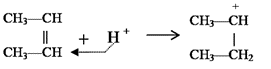
\includegraphics[height=2.3 cm]{fig1.png}
\caption{The addition of an acid proton to an olefin to produce a \emph{tert}-butyl carbation}
\label{fig1}
\end{figure}

2. In the second stage, the formed carbonium ion interacts with paraffin hydrocarbon. In this case, the hydrogen anion from the tertiary carbon atom of the isoparaffin hydrocarbon passes into the carbonium ion formed in the first stage of the reaction:

\begin{figure}
\centering
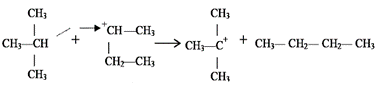
\includegraphics[height=3.3 cm]{fig2.png}
\caption{The interaction of the formed carbonium ion with paraffin hydrocarbon}
\label{fig2}
\end{figure}

3. The third stage consists of the addition of a tertiary carbonium ion to the second olefin molecule to form carbonium:

\begin{figure}
\centering
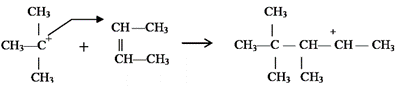
\includegraphics[height=3.3 cm]{fig3.png}
\caption{The addition of a tertiary carbonium ion to the second olefin molecule}
\label{fig3}
\end{figure}

4. The fourth stage consists of the skeletal isomerization of the secondary carbonium ion:

\begin{figure}
\centering
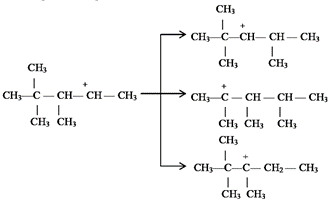
\includegraphics[height=6.3 cm]{fig4.png}
\caption{The skeletal isomerization of the secondary carbonium ion}
\label{fig4}
\end{figure}

5. The fifth stage is the interaction of the formed carbonium ions with an isoparaffin molecule by a tertiary carbon-hydrogen bond with the formation of target products and a carbonium ion from isoparaffin:

\begin{figure}
\centering
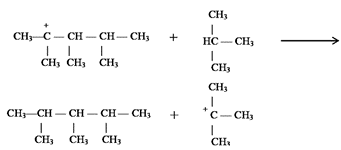
\includegraphics[height=3.5 cm]{fig5.png}
\caption{The interaction of the formed carbonium ions with an isoparaffin molecule}
\label{fig5}
\end{figure}

For ease of use when compiling the model, we offer below a scheme containing the reactions in the sulfuric acid alkylation process (Fig.\,\ref{fig6}).

\begin{figure}
\centering
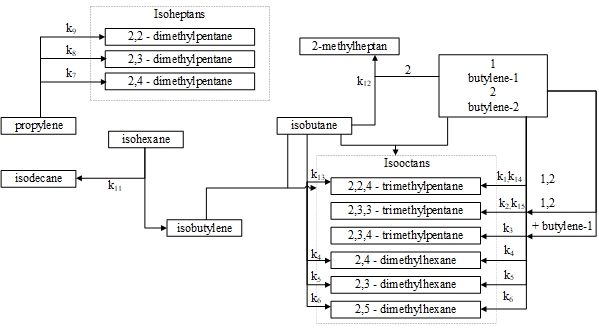
\includegraphics[height=6.5 cm]{fig6.png}
\centering
\caption{The scheme of reactions of the sulfuric acid alkylation process}
\label{fig6}
\end{figure}

It should be noted that the temperature range of the process is from 2\,\textcelsius{} to 15\,\textcelsius{}. Determining the optimal value for a given composition of feedstocks is one of the study objectives. The solution to the problem of constructing a model of the process of sulfuric acid alkylation of isobutane with butylenes is relevant in this regard~\cite{alkylation_mod}.

%Ñòûêîâî÷íûé àáçàö
Since the mathematical model of the chemical reaction is a system of differential equations, it is only possible to find the values of the constants in this system numerically (see, e.g., \cite{Gubaydullin2021}). Note that the objective function in such problems is usually multiextremal, i.e., it has many local extrema apart from the global one.

%×àñòü ÍÍÃÓ
%The numerical methods for solving such multiextremal problems (global optimization methods) differ significantly from local search methods (see, e.g., \cite{PaulaviciusZilinskas2014,Sergeyev2017}). From an algorithmic point of view, they can be divided into two classes: metaheuristic and deterministic. Metaheuristic algorithms are mainly based on the simulation of processes occurring in living nature. Typical examples of such algorithms are simulated annealing, evolution and genetic algorithms, and others (see, e.g., \cite{Battiti2009,Eiben2015}). Owing to their relative simplicity, metaheuristic algorithms are more popular with researchers than deterministic ones. However, the solution to a problem found by a metaheuristic algorithm is, generally speaking, local and may be well away from the global solution \cite{Kvasov2018}.

Assuming some additional properties of the objective function, it is possible to construct efficient deterministic methods for finding a global solution. For example, we can assume that the ratio of the function increment to the corresponding argument increment can not exceed some threshold. In this case, the functions are called Lipschitzian, and the problem itself is a Lipschitz optimization problem.
This paper continues a series of papers where the parallel methods of Lipschitz optimization proposed in \cite{Strongin2000} are investigated and modified in their application to solving inverse problems of chemical kinetics.

The main part of the paper is organized as follows. Section \ref{Sec_math_mod} describes the mathematical model of the chemical reaction under study. The formal statement of the Lipschitz global optimization problem and the general scheme of the search for algorithms are given in Section \ref{Sec_GSA}. In that section, we also present a scheme of the proposed asynchronous parallel algorithm for solving multiextremal problems. The results of the numerical solution of the inverse problem of chemical kinetics are discussed in Section \ref{Sec_Exp}.

\section{The Problem Statement} \label{Sec_math_mod}

To optimize the technological process, it is necessary to know the kinetic laws and mechanisms of chemical reactions. To determine them, we should evaluate the kinetic parameters of chemical reactions by solving the inverse problem of chemical kinetics~\cite{regularization}. In most cases, the equations of chemical kinetics are systems of ordinary nonlinear differential equations for the concentrations of substances $x_{i}$ (\ref{concentration_changing}) with initial conditions (\ref{init_cond}):
\begin{gather}
  \frac{dx_{i}}{dt} = \sum_{j=1} ^J \nu_{ij} \omega_j,\quad i=1,\ldots.I,\ \omega_j=k_j^0 \cdot \exp \biggl(-\frac{E_{j}}{RT}\biggr)\cdot \prod_{i=1} ^M x_{i}^{|a_{ij}|},
\label{concentration_changing}\\
t=0,\ x_i(0)=x_i^0.
\label{init_cond}
\end{gather}
Here $k_j^0 \cdot \exp\bigl(-\frac{E_{j}}{RT}\bigr)$ are the so-called rate constants of the reaction stages; $I$ is the number of substances involved in the reaction; $J$ is the number of reaction stages; $\nu_{ij}$ are stoichiometric coefficients; $E_j$ are the activation energies of the reactions (cal/mol); $R$ is the universal gas constant (cal/(mol $\cdot$ K)); $T$ stands for the temperature (K); $a_{ij}$ are the stoichiometric coefficients; $k_j^0$ are pre-exponential multipliers.

The inverse problem of chemical kinetics is a global optimization problem implying the need to determine the vector of reaction rate constants $(k_1, k_2, \ldots, k_J)$ at which the deviation of the calculated concentrations of the reaction components from the experimental ones is minimal.
Thus, to determine the rate constants of the reaction, it is necessary to solve the inverse problem of chemical kinetics by repeatedly solving the direct problem, that is, by iterating over the rate constants of the stages (or a set of pre-exponents and activation energies) according to some algorithm. To solve the optimization problem, it is necessary to minimize the functional (\ref{functional}), which expresses the deviation of experimental data from the calculated values:
\begin{equation}
FF = \sum_{i=1} ^M \sum_{j=1} ^N |x_{ij}^{\mathrm{calc}} - x_{ij}^{\mathrm{exp}}|.
\label{functional}
\end{equation}
Here $x_{ij}^{\mathrm{calc}}$ are the calculated values, $x_{ij}^{\mathrm{exp}}$ are experimental data, $M$ is the number of experimental points, and $N$ is the number of substances involved in the reaction.
To solve the instability issue in optimization problem (\ref{functional}), consider the minimization problem in the general form
\begin{equation}
f(z) \rightarrow \inf,\quad z \in D,
\label{problem}
\end{equation}
where $D$ is some given set and $f\colon D \rightarrow R^1$ is a function (functional) defined on it.

In this inverse problem of chemical kinetics, a number of kinetic parameters act as a point $z$ (as a rule, a vector of reaction rate constants), while the function $f$ is the deviation of the calculated concentrations of the reaction components from empirical data (functional (\ref{functional})).
Problem (\ref{problem}) can be attributed to one of two classes of problems, which in the literature are called correctly posed and incorrectly posed minimization tasks, respectively. Inverse problems of chemical kinetics are \emph{incorrectly posed problems}  (or, in other words, \emph{ill-posed problems}). According to Hadamard, a problem is considered to be \emph{correctly posed} if: 1) its solution exists, 2) the solution is unique, and 3) the solution is stable to variations in the initial data. If at least one of the listed requirements does not hold, the task is considered incorrectly posed. The inverse problems of chemical kinetics encountered in practice usually have a solution, and condition 1 is, thus, fulfilled. Most often, however, conditions 2 and 3 do not hold~\cite{regularization}.
To solve ill-posed problems approximately, we need special methods to construct a solution to problem (\ref{problem}). Such methods exist and are commonly called regularization methods. In this paper, we rely on a regularization method suggested by A.\,N.~Tikhonov and called the \emph{stabilization method}. Also, we use the classical machine-learning apparatus, i.e., normalization of features and scaling.
The main task that we will consider is the minimization problem
\begin{equation}
f^0(z) \rightarrow \inf,\quad z \in D \subset Z,
\label{minimization_problem}
\end{equation}
in which we assume $D$ to be a convex closed set in a Hilbert space $Z$. The function $f^0\colon D \rightarrow R^1$ is considered continuous and convex on $D$. Suppose that problem (\ref{minimization_problem}) has a solution, i.e., the set $D^*$ is nonempty. Denote by $z^0$ the norm-minimal solution to the problem. Suppose that instead of an exact function $f$, we know its approximation $f_{\delta}$, where $\delta \in [0, \delta_0], \delta_0>0$, is a sufficiently small number, and, moreover,
\begin{equation}
|f^\delta(z) - f^0(z)| \leq \delta (1+||z||^2),\quad  \forall z \in D.
\end{equation}

The main construction of the Tikhonov method is the smoothing function or Tikhonov function
\begin{equation}\label{formula_T}
T_\alpha^\delta(z) \equiv f^\delta(z) + \alpha \lVert z\rVert^2,\quad z \in D,
\end{equation}
where $\alpha > 0$ is the regularization parameter; $\alpha||z||^2$ is called the stabilizing term. Consider the auxiliary minimization problem
\begin{equation}
T_\alpha^\delta(z) \rightarrow \inf,\quad z \in D.
\label{tikhonov_F}
\end{equation}
Various numerical methods can be applied to approximate the solution of this problem. Suppose that, as a result of a finite number of iterations, we obtain a point $z_\alpha^{\delta,\epsilon}$ such that
\begin{equation}
T_\alpha^\delta(z) \equiv \min T_{\alpha}^{\delta}(z) \leq T_{\alpha}^{\delta} (z_{\alpha}^{\delta,\epsilon}) \leq T_{\alpha}^{\delta} + \epsilon,
\end{equation}
where $\epsilon > 0$ is a number that characterizes the accuracy of the solution to minimization problem (\ref{tikhonov_F}). In this case, minimization problem (\ref{tikhonov_F}) for each fixed pair $\delta, \alpha$ has, as a rule, a much larger ``margin of stability'' than the original problem (\ref{problem}) and, in most cases, is correctly posed.

\section{The Parallel Global Optimization Algorithm}\label{Sec_GSA}

\subsection{The Optimization Problem}\label{Sec_GO_Problem}

As we mentioned above, the task of identifying the model parameter values can be considered a Lipschitz global optimization problem. From a formal point of view, this problem is a mathematical programming problem of the form
\begin{equation} \label{problemN}
 \varphi^* = \varphi(y^\ast)=\min{\left\{\varphi(y):y\in D\right\}},
 \end{equation}
\begin{equation} \label{D}
 D=\left\{y\in R^N : a_i\leq y_i \leq b_i, \;  1\leq i \leq N\right\},
 \end{equation}
where the vectors $a,b\in R^N$ correspond to the lower and upper bounds of the search region, and $\varphi(y)$ is the objective function, which satisfies the Lipschitz condition
\begin{equation}\label{Lip}
\left|\varphi(y_1)-\varphi(y_2)\right|\leq L\lVert y_1-y_2\rVert,\quad
y_1,y_2 \in D.
\end{equation}

We assume that the function $\varphi(y)$ is multiextremal and is given as a ``black box'' (i.e., as some subroutine with a vector of parameters as its input and the calculated value of the function as its output). Moreover, we suppose that each application of this procedure (hereinafter referred to as a \emph{search trial}) is a time-consuming operation. This formulation of the problem is fully consistent with the inverse problem of chemical kinetics.

There are several algorithms that can be applied to solve Lipschitz optimization problems. These include, among others, the nonuniform covering method \cite{Evtushenko2009,Evtushenko2013}, and diagonal and simplicial partition methods \cite{Zilinskas2010,Paulavicius2011}. In this paper, we rely on the global search algorithm proposed by Strongin \cite{Strongin2000}. Under this approach, the original multidimensional problem (\ref{problemN}) is reduced to a one-dimensional optimization problem using Peano-Hilbert curves.

In fact, using a continuous one-to-one mapping (Peano curve) $y(x)$ of the segment $[0,1]$ of the real axis onto the hyperinterval $D$ in (\ref{D}), we can reduce the original problem (\ref{problemN}) to the one-dimensional problem
\[
\varphi(y^\ast)=\varphi(y(x^\ast))=\min{\left\{\varphi(y(x)): x\in[0,1]\right\}},
\]
where the one-dimensional function $\varphi(y(x))$ satisfies the H{\"o}lder condition
\[
\left|\varphi(y(x_1))-\varphi(y(x_2))\right|\leq H\left|x_1-x_2\right|^{1/N}
\]
with $ H=2 L \sqrt{N+3}$.
The numerical construction of various approximations of such mappings is discussed in \cite{Sergeyev2013,Strongin2000}.

Thus, the search trial at some point $x'\in[0,1]$ will involve, in the first place, the construction of the image $y'=y(x')$ and only then the computation of the function value $z' = \varphi(y')$.

\subsection{Characteristic Algorithms}

%Õàðàêòåðèñòè÷åñêèé àëãîðèòì
The global search algorithm we use belongs to the class of \emph{characteristic algorithms}, and this greatly simplifies the process of its parallelization. Recall that a numerical optimization method belongs to the class of characteristic algorithms if the algorithmic scheme of this method can be described as follows.

At the first iteration, the trials are performed at the points $x^1 = 0$ and $x^2 = 1$. Then, each following $(k+1)$-th, $k \geq 2$, iteration of the global search is executed as described below.
\begin{enumerate}
	\item
Renumber the points of the previous trials by increasing their $x$-coordinates (the new order is determined by the subscripts):
\[
0=x_0<x_2<\ldots<x_{k}=1.
\]

	\item
For every interval $(x_{i-1},x_i), 1\leq i\leq k$, we calculate a value $R(i)$ called the \textit{interval characteristic}. In the general case, $R(i)$ can depend on the points $x^i$ and the trial results $z^i=f(x^i)$, $1 \leq i \leq k$.

	\item
Find the interval $(x_{t-1},x_t)$ with the largest characteristic $R(t)$, i.e.,
\[
R(t) = \max \left\{ R(i) : 1\leq i\leq k \right\}.
\]

	\item
Examine the stop condition
\[
\Delta_t \leq \epsilon ,
\]
where $\epsilon>0$ is a given accuracy. If the stop condition is satisfied, then the global search should be terminated; otherwise, the calculations continue.

	\item
Select a point $x^{k+1}$ of the current iteration within the interval $(x_{t-1},x_t)$ in accordance with some rule $S(t)$, i.e.,
\[
x^{k+1} = S(t)\in(x_{t-1},x_t).
\]
	
	\item
Calculate the function value $z^{k+1} = f(x^{k+1})$.

	\item
Evaluate a global minimum estimate.

	\item
Increase the iteration number $k=k+1$ and proceed to the next iteration.
\end{enumerate}

As a possible interpretation of this scheme, we can consider the interval characteristic $R(i)$ as a measure of the global minimum being within the interval
$(x_{i-1},x_i)$.
To construct a concrete form of the interval characteristic, we can use a lower envelope (or minorant) of the function to be minimized or a mathematical expectation of the function values, etc.
Most well-known global optimization methods can be formulated in accordance with this characteristic scheme, e.g.,
\begin{itemize}
\item uniform grid methods with a successively reduced step;
\item random search (Monte Carlo) algorithms;
\item the Piyavskii algorithm \cite{Piyavskii1972};
\item one-step Bayesian algorithms proposed by Kushner and \v{Z}ilinskas \cite{Zilinskas1989};
\item information algorithms proposed by Strongin \cite{Strongin2000}.
\end{itemize}
All these methods are based on different mathematical models but are presented in a general characteristic scheme.

It should also be noted that the length of the interval with the largest characteristic is examined at the stop condition.
It is possible if the optimization method converges to the global minimum.
The details of these methods are given in the cited sources.
%Çäåñü æå îòìåòèì îñíîâíûå ìîìåíòû
Here we highlight the main points.

For the Piyavskii method, the interval characteristic $R(i)$ is an estimate (with the inverse sign) of the minimum value of the objective function $f(x)$ in the interval $(x_{i-1},x_i)$. As a result, the point of a new trial is taken within the interval containing the estimate of the minimum value of $f(x)$ over the search domain.

The Kushner technique and the \v{Z}ilinskas method are constructed in the framework of the approach when the objective function is regarded as
a sample of some Wiener process. For the Kushner technique, the point $x^{k+1}$ of the current iteration is the most probable point at which the function value
$f(x^{k+1})$ is not greater than the value
\[
z_k^* -\gamma (z_k^+-z_k^*),
\]
where $z_k^+$ and $z_k^*$ are estimates of the function maximum and minimum values, respectively. For the \v{Z}ilinskas method, $x^{k+1}$ is the point where the maximum average improvement of the current estimate of the global extremum is expected.

The Strongin global search algorithm is constructed in the framework of the information approach to global optimization (see \cite{Strongin2000}). This method has an adaptive scheme to evaluate the numerical estimate of the unknown Lipschitz constant.

\subsection{Parallel Algorithm with Asynchronous Trials}\label{Sec_PGSA}

The global search algorithm (GSA) belongs to the class of characteristic algorithms; this fact suggests a possible way to parallelize it.
As previously mentioned, the interval characteristic $R(i)$ can be regarded as some measure of finding the global minimum point in the given interval. Then, instead of a single best interval, several intervals with the highest characteristics can be chosen at once, and successive trials can be carried out in these intervals in parallel. Moreover, the scheme of characteristic algorithms also allows for asynchronous parallelization, which minimizes the downtime of processors when the trial complexity depends on a particular point in the search domain.

Let us now examine the parallel algorithm with asynchronous trials in more detail. It implements a parallel scheme of the ``master/worker'' type. The master process accumulates search information, evaluates on its basis the Lipschitz constant for the target function, determines new trial points, and sends them to the worker processes. Worker processes receive points from the master, carry out new trials at these points, and send the results to the master.

When describing the parallel algorithm, we assume that there are $p+1$ computational processes: one master and $p$ worker processes.

At the beginning of the search, the master process (let it be process number 0) initiates $p$ parallel trials at $p$ different points of the search domain, two of which are boundary points and the rest are internal points, i.e., at the points $\{y(x^1), y(x^2), \ldots,y(x^p)\}$, where $x^1 = 0$, $x^p = 1$, $x^i\in(0,1)$, $i=2,\ldots, p-1$.

Suppose now that $k$ trials have been performed (in particular, $k$ can be 0), and the worker processes perform trials at points $\{y(x^{k+1}), y(x^{k+2}), \ldots,y(x^{k+p})\}$.

If a worker process completes the trial at some point (let it be the point $y(x^{k+1})$, corresponding to process number 1), then it sends the results of the trial to the master process. Note that, in this case, we have a set of inverse images of the trial points
\[
S_k = \left\{ x^{k+1},x^{k+2},\ldots,x^{k+p} \right\},
\]
where the trials have already started but are not completed yet.

After receiving the trial results at the point $y(x^{k+1})$ from the worker process, the master selects a new trial point $x^{k+p+1}$ for it, according to the rules corresponding to the scheme of the characteristic algorithm.
\begin{enumerate}
	\item
Renumber the set of inverse images of the trial points
\[
X_k = \left\{x^1, x^2,\ldots,x^{k+p} \right\},
\]
which contains all inverse images at which the trials have either been carried out or are being carried out, arranged in an ascending order (determined by the subscripts), i.e.,
\[
0=x_1<x_2<\ldots<x_{x+p}=1.
\]

	\item
Calculate the values
\[
\begin{aligned}
M_1&=\max \left\{ \frac{ \left|z_i - z_{i-1} \right|}{(x_i-x_{i-1})^{1/N}} : x_{i-1} \notin S_k, x_i \notin S_k, 2\leq i\leq k+p \right\},\\
M_2&=\max \left\{ \frac{ \left|z_{i+1} - z_{i-1} \right|}{(x_{i+1}-x_{i-1})^{1/N}} : x_i \in S_k, 2\leq i < k+p \right\},\\
M&=\max\{M_1,M_2\},
\end{aligned}
\]
where $z_i=\varphi(y(x_i))$ for all $x_i \notin S_k$.
%The values of $z_i$ at the points $x_i \in S_k$ are undefined, as the trials at these points have not yet been completed.
If $M$ equals 0, then assume $M=1$.

	\item
Assign to each interval $(x_{i-1},x_i)$, $x_{i-1} \notin S_k$, $x_i \notin S_k$, the characteristic $R(i)$, calculated by the formula
\begin{equation} \label{R}
R(i)=rM\Delta_i+\frac{(z_i-z_{i-1})^2}{rM\Delta_i}-2(z_i+z_{i-1}),
\end{equation}
where $r>1$ is a method parameter and $\Delta_i=\left(x_i-x_{i-1}\right)^{1/N}$.

	\item
Find the interval $[x_{t-1},x_t]$ to which the maximum characteristic corresponds, i.e.,
\[
R(t) = \max \left\{ R(i) : x_{i-1} \notin S_k, x_i \notin S_k, 2\leq i\leq k+p \right\}.
\]

	\item
Determine the inverse image $x^{k+p+1} \in (x_{t-1},x_t)$ of the new trial point by the formula
\[
x^{k+p+1} = \frac{x_{t}+x_{t-1}}{2} - \operatorname{sign}(z_{t}-z_{t-1})\frac{1}{2r}\left[\frac{\left|z_{t}-z_{t-1}\right|}{M}\right]^N.
\]
\end{enumerate}

Immediately after calculating the next trial point $y^{k+p+1} = y(x^{k+p+1})$, the master process adds it to the set $S_k$ and forwards it to the worker process, which initiates a trial at this point.

The master process completes the algorithm when one of two conditions holds: $\Delta_{t}<\epsilon$ or $k+p>K_{\mathrm{max}}$.
The first one corresponds to stopping the algorithm by accuracy, and the second one, by the number of trials. The real number $0<\epsilon<1$ and the integer $K_{\mathrm{max}}>0$ are algorithm parameters.

\section{Numerical Experiments} \label{Sec_Exp}

To determine the constants of the process reactions, it is necessary to solve a system of differential equations that describes the change in the concentrations of the reaction components over time \cite{cao2019}.

In preliminary experiments, we estimated the approximate time to calculate one objective function using the corresponding sequential algorithm. The computer architecture used for the experiments was based on Intel\textsuperscript{\tiny\textregistered} Core\textsuperscript{\tiny\texttrademark} i7-10750H processors at 2.60~GHz. The average computation time of the objective function was about $0.2$ sec, which characterizes the problem as being computationally complex. Solving the problem with the sequential algorithm would require no less than 1 million trials, that is, at least 54 hours (as an estimate). Therefore, only the parallel algorithm with a stopping criterion based on the number of trials $K_{\mathrm{max}}=10^6$ was used for the calculations.

The numerical experiments were performed with the parallel asynchronous algorithm outlined in Section \ref{Sec_PGSA}, running 160 processes: 159 processes calculated the values of the objective function (worker processes), and one master process controlled the algorithm. The experiments were conducted on the Lobachevsky supercomputer, installed at the University of Nizhni Novgorod. The asynchronous global optimization algorithm was implemented in C++ (with GCC 9.5.0 and Intel MPI). The computation of the objective function values was implemented in Python 3.9.

\begin{table}
\caption{Dependence of the function minimum value $\varphi^*$ on the regularization parameter $\alpha$}
\label{table_1}
\begin{center}
\begin{tabular}{c@{\quad}cc}
\hline\noalign{\smallskip}
 $\alpha$      & $\varphi^*$  & Time (sec.) \\
\hline\noalign{\smallskip}
0.0\PhUnit{00} &	0.573920 & 838.9	\\
0.001	&	0.540750	&	853.9	\\
0.002	&	0.547907	&	850.0	\\
0.003	&	0.583529	&	831.5	\\
0.004	&	0.579725	&	821.4	\\
0.005	&	0.615638	&	815.4	\\
0.006	&	0.612614	&	834.7	\\
0.007	&	0.619546	&	807.3	\\
0.008	&	0.604817	&	830.4	\\
0.009	&	0.630010	&	814.4	\\
0.01\PhUnit{0}	&	0.632944	&	825.2	\\
0.02\PhUnit{0}	&	0.669092	&	155.8	\\
0.03\PhUnit{0}	&	0.681520	&	809.2	\\
0.04\PhUnit{0}	&	0.736035	&	816.4	\\
0.05\PhUnit{0}	&	0.729415	&	804.7	\\
0.07\PhUnit{0}	&	0.759134	&	803.6 \\
0.06\PhUnit{0}	&	0.723404	&	810.9	\\
0.08\PhUnit{0}	&	0.808238	&	811.8	\\
0.09\PhUnit{0}	&	0.837868	&	828.6 \\
0.1\PhUnit{00}	&	0.810454	&	806.2	\\
\noalign{\smallskip}\hline
\end{tabular}\end{center}\end{table}

%Óñêîðåíèå ñîñòàâèëî ïðèìåðíî $230$ ðàç.
The short time obtained when solving the problem by the parallel algorithm (approximately 14 minutes per problem) made it possible to investigate thoroughly the dependence of the solution on the regularization parameter $\alpha$. Table \ref{table_1} shows the minimum values of the objective function found for the corresponding value of the regularization parameter and the time for solving the problem (in seconds).
%and the time speedup in comparison to the estimated problem solution time when using the sequential method.
The algorithm was run with the method parameter $r=4.0$ from (\ref{R}) and the accuracy $\epsilon = 10^{-4}\left\|b-a\right\|$. After a given number of iterations or after reaching the specified accuracy with the global search method, the solution was refined by the Hooke--Jeeves local method \cite{HookJeeves} with the accuracy $\epsilon = 10^{-4}\left\|b-a\right\|$.

A detailed study of the region of the regularization parameter values in a neighborhood of $\alpha=0$ (from $0.1$ to $0.01$ with steps of $0.01$ and from $0.01$ to $0.001$ with steps of $0.001$) showed that the value of the minimum decreases as $\alpha$ decreases. The best solution, equal to $0.54075$, was obtained with the regularization parameter $\alpha = 0.001$.

In the course of the research, we calculated the functional $f(z)$ without taking into account the addition of the regularization term (Fig.\,\ref{fig7}). Afterward, we carried out a similar calculation taking into account the regularization term. The results for $\alpha=0.002$ were $0.527$ without regularization and $0.547$ with regularization.

\begin{figure}
\centering
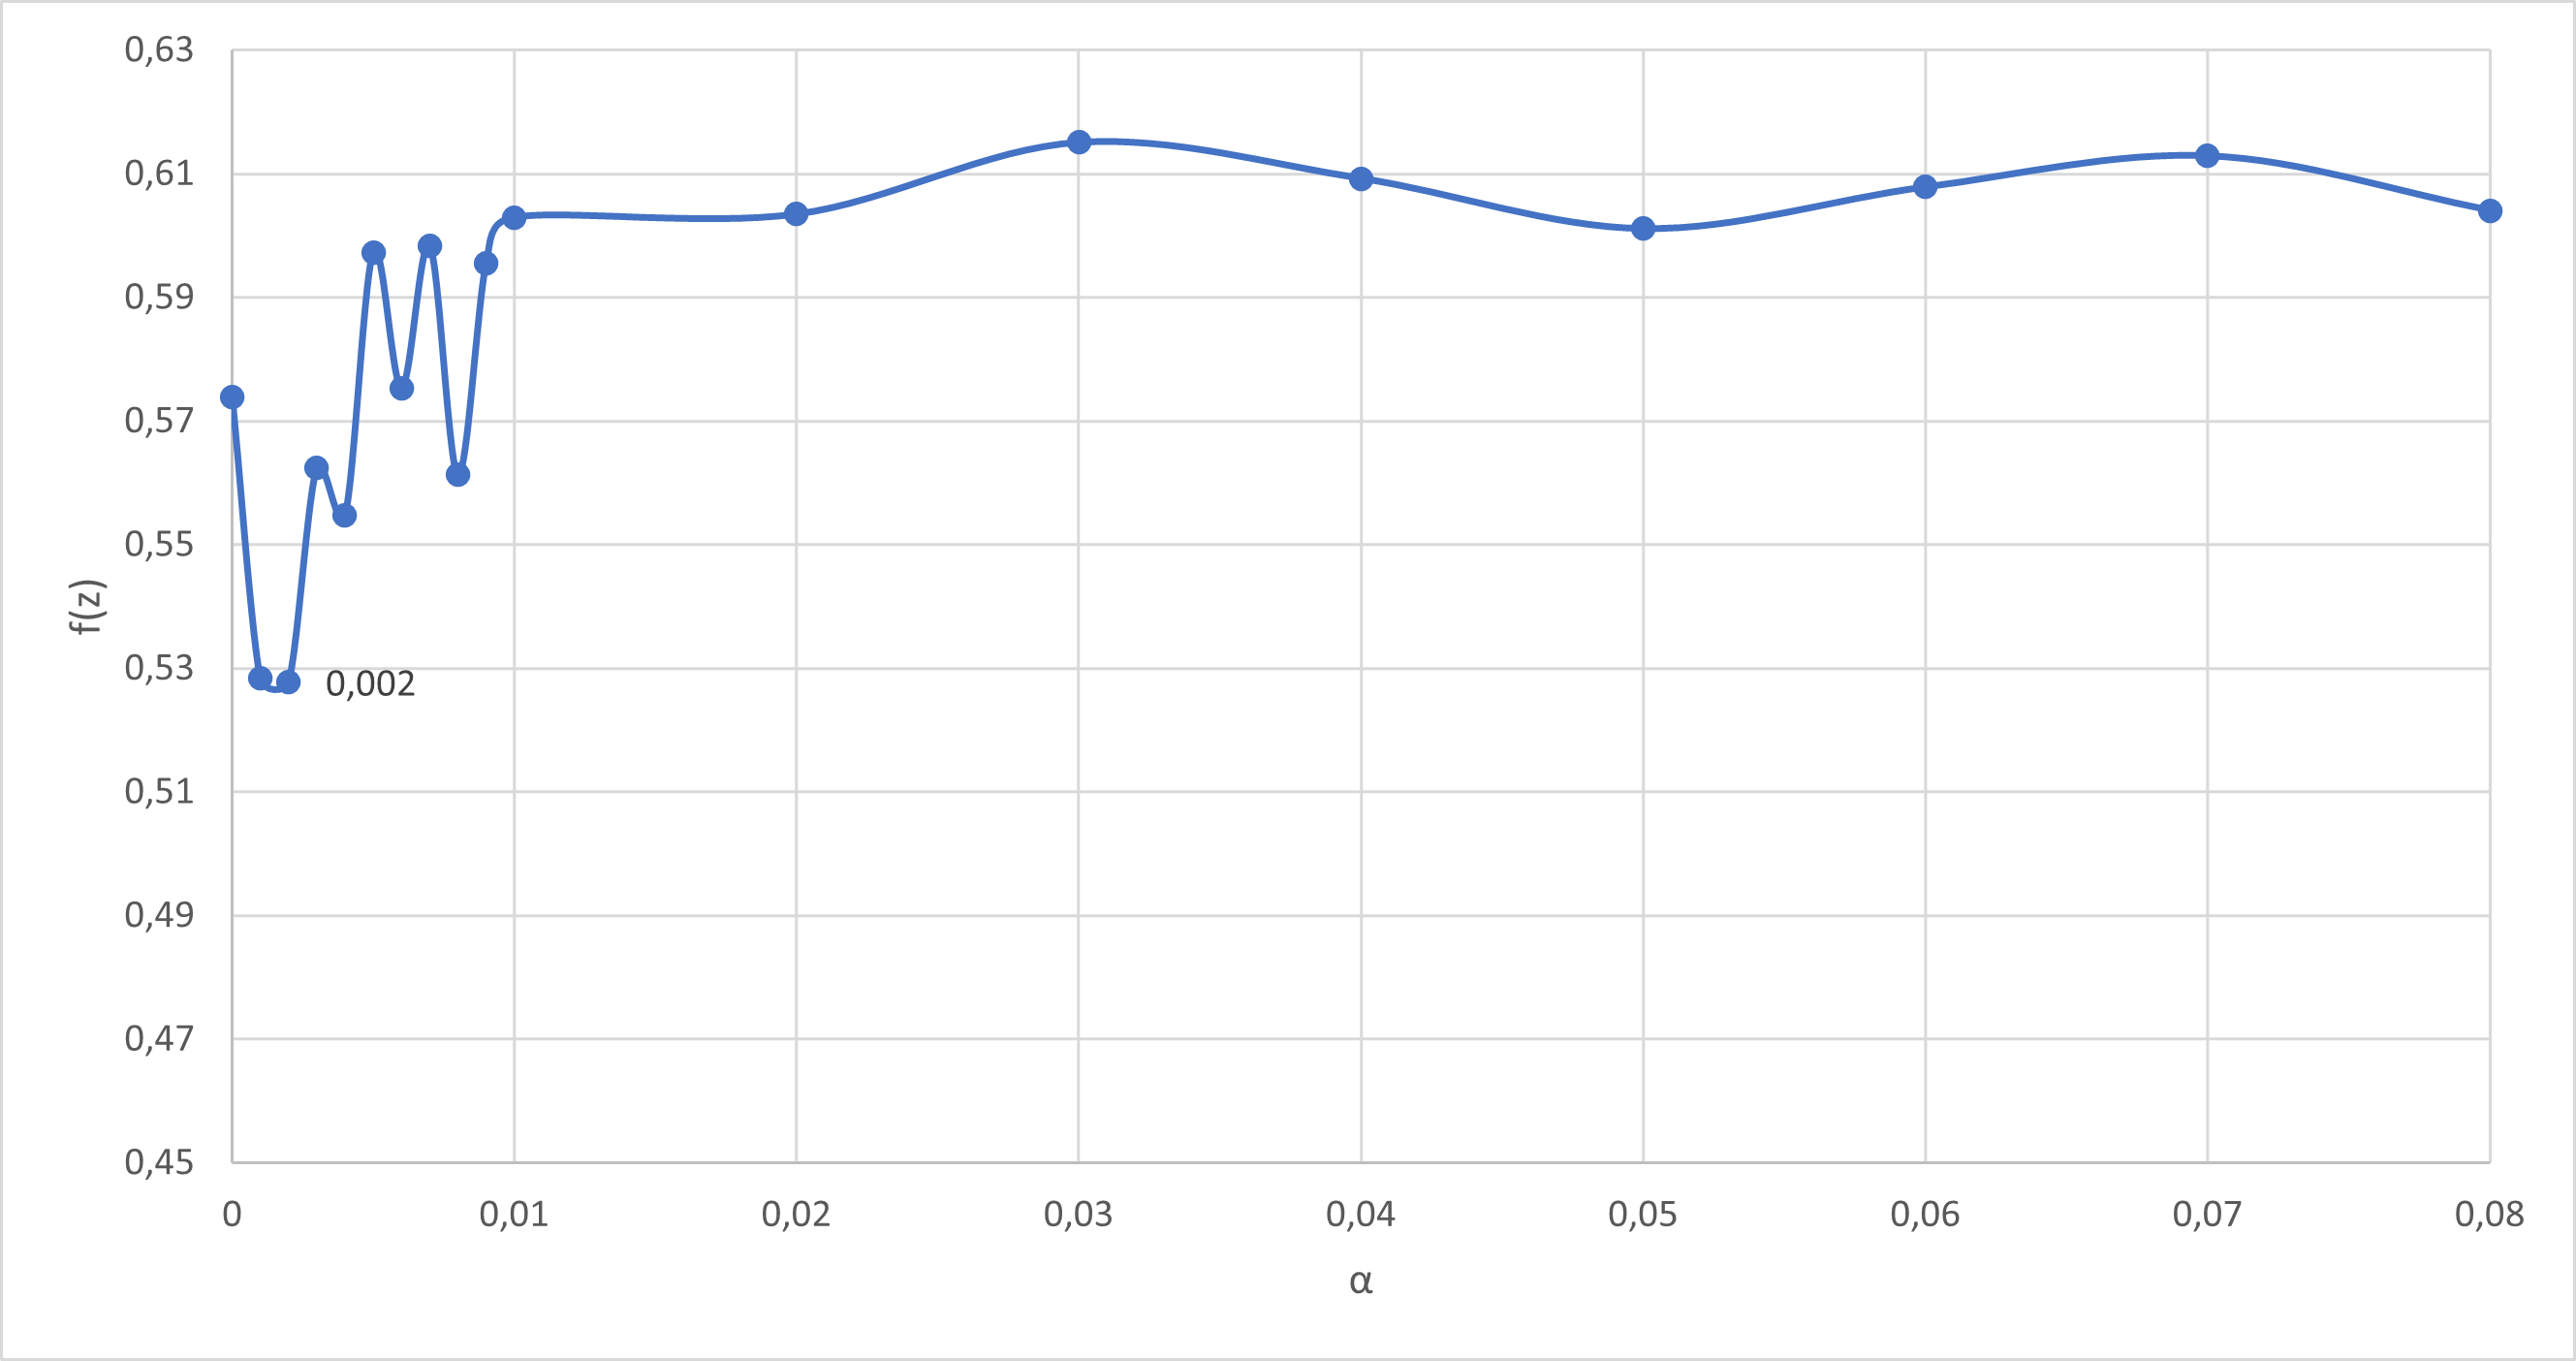
\includegraphics[height=6.0 cm]{fig7.png}
\caption{The value of the functional $f(z)$ without taking into account the addition of the regularization term}
\label{fig7}
\end{figure}

The speedup of the parallel global optimization algorithm was estimated for the problem to which the best solution was found, i.e., the problem with regularization parameter $\alpha = 0.001$.
Since solving the problem in serial mode would require about two days, the speedup was evaluated with respect to a parallel launch involving a smaller number of processes.
Table \ref{table_2} shows the running time and speedup of the parallel algorithm using 80 and 160 processes with respect to the running time on 40 processes.

\begin{table}
\caption{The speedup of the parallel global optimization algorithm}
\label{table_2}
\begin{center}
\begin{tabular}{ccc}
\hline\noalign{\smallskip}
 $p$     & Time (sec.)  & Speedup \\
\hline\noalign{\smallskip}
\PhUnit{0}40	&	2778.7		&	--	\\
\PhUnit{0}80	&	1495.5		&	1.9	\\
160	&	\PhUnit{0}853.9	    &	3.3	\\
\noalign{\smallskip}\hline
\end{tabular}\end{center}\end{table}

\section{Conclusions}

We solved in this paper an incorrectly posed problem using the Tikhonov regularization method and found the reaction constants of the process of sulfuric acid alkylation of isoalkanes by alkenes. The optimization method allowed us to find an accurate description of the experimental data. The authors plan to use the Tikhonov regularization method in forthcoming research to build kinetic models of other chemical processes.

The parallel global search algorithm showed good results. The solution to the problem was obtained in approximately 15 minutes on the Lobachevsky supercomputer; the estimated time for solving the same problem with the corresponding sequential algorithm was more than 50 hours. The experiments were conducted using 160 processes on the supercomputer nodes. However, an increase in the dimension of the considered global optimization problem (in the case of complex inverse problems of chemical kinetics, the number of parameters can be hundreds) leads to a decrease in search quality.

A possible topic for further research is the development of methods for analyzing the accumulated search information to identify groups of parameters that have little effect on the objective function. To find the optimal values of such parameters, it is sufficient to employ local optimization methods. The analysis can rely, for example, on machine-learning methods. In this case, the cost of solving the whole problem decreases, and it becomes feasible to obtain the global solution with good accuracy in an acceptable time.

\subsubsection*{Acknowledgments.}
%This study was supported by the Ministry of Science and Higher Education of the Russian Federation (project no. FSWR-2023-0034), and by the Research and Education Mathematical Center (project no. 075-02-2022-883). This research was partially funded by the state task of the Institute of Petrochemistry and Catalysis of the Russian Academy of Sciences (theme No. FMRS-2022-0078).

%This research was partially funded by the Ministry of Science and Higher Education of the Russian Federation (project \textnumero~FSWR-2023-0034), the Research and Education Mathematical Center (project \textnumero~075-02-2022-883; development of the parallel global optimization algorithm), and the Ministry of Science and Higher Education of the Russian Federation (project \textnumero~FMRS-2022-0078; investigation of the chemical kinetics problem).

This research was partially funded by the projects \textnumero~FSWR-2023-0034, \textnumero~075-02-2022-883 (development of the parallel global optimization algorithm), and by the project \textnumero~FMRS-2022-0078 (investigation of the chemical kinetics problem).


%
% ---- Bibliography ----
%
\bibliographystyle{spmpsci}
\bibliography{example-bibtex}{}

\end{document}
